\documentclass[10pt,a4paper]{article}
\usepackage[margin=2.2cm]{geometry}
\usepackage[T1]{fontenc}
\usepackage[utf8]{inputenc}
\usepackage{amsmath,amssymb,booktabs,array,graphicx}
\usepackage{tikz,pgfplots}
\usetikzlibrary{arrows.meta,positioning,shapes.geometric}
\pgfplotsset{compat=1.18}
\usepackage[colorlinks=true,urlcolor=blue,citecolor=blue,linkcolor=blue]{hyperref}
\usepackage{microtype}
\setlength{\parskip}{3pt}
\title{Selective Adaptation to Communication and Actuation Shifts\\in Cooperative Multi-Agent Reinforcement Learning}
\author{Working manuscript: authors and affiliations to be confirmed}
\date{Version 0.2 --- 29 September 2026\\\small Closed descriptive study; three LIAM training seeds}
\begin{document}
\maketitle
\begin{abstract}
Cooperative agents may fail because received messages change meaning or because movement commands change effect. We study whether correcting these two interfaces separately helps a frozen recurrent policy recover. Our system, V2, combines a learned message translator with a motor module that estimates command effects from observed motion. A gate enables message correction only after evidence of a change; a trial disables it if returns worsen. We evaluate message permutations, actuator rotation, both changes, and no change in a two-agent particle task. In a completed five-seed control study, selective activation did not outperform simpler correction rules according to the planned criterion. A separate comparison with a port of the official LIAM implementation was closed after three of five planned seeds because of interrupted server access and the project deadline. V2 has higher mean post-change returns in all four conditions, but LIAM performs better after message changes in two seeds; its weak third seed affects the aggregate ranking. Motor correction restores much of the frozen policy's performance, whereas the benefit of selective message correction remains unproven. We report unequal intervention scope and training resources, and propose experiments to distinguish decoding errors, delayed activation and an uncorrected partner.
\end{abstract}

\section{Introduction}
Cooperating agents can fail for distinct reasons: a received symbol may acquire a different interpretation, or a familiar motor command may produce an unexpected displacement. A policy can observe lower reward under either change. Deciding which component to modify is therefore separate from detecting that performance has declined. We examine whether explicit separation of receiver correction and actuator correction is useful, and whether selectively enabling these corrections improves on simpler rules.

We separate where corrections act: message correction changes the policy input, whereas motor correction changes its movement output. This does not imply that the neural network learns independent representations of meaning and movement. Our implementation combines a pretrained recurrent policy, a supervised message memory, and a small online motor-identification module. No neural weights are updated during the evaluated deployment sessions. We contribute an intervention harness, reproducible comparisons, and an analysis of when this decomposition helps or fails. The results currently do \emph{not} establish that selective routing is necessary or superior.

We distinguish three questions: (Q1) does correction improve on the frozen policy; (Q2) does selective routing improve on simpler correction rules; and (Q3) how does this system compare with a published local-information agent-modelling method under the same evaluation interface? These questions require different controls. Success on Q1 does not answer Q2 or Q3.

\section{Related work and scope}
Multi-agent actor--critic methods provide a foundation for cooperative policies with decentralized execution \cite{lowe2017}. We use an implementation of recurrent MAPPO associated with the cooperative PPO study of Yu et al.\ \cite{yu2022}, rather than developing a new policy optimizer. Our environment extends MPE2 Simple Reference \cite{mpe2}; we retain its particle dynamics and add controlled interventions.

LIAM infers a compact representation from an agent's local history and uses it to condition its policy. During training, the other agent's observations and actions supervise reconstruction; these targets are unavailable at execution \cite{papoudakis2021}. Our comparator imports the released LIAM core \cite{liamcode}. It is a published specialized comparator, not a proxy for every contemporary state-of-the-art method. We have not reproduced the original paper's benchmark scores.

\section{Task and intervention harness}
\subsection{Native environment}
Two agents communicate to navigate toward three landmarks, using information supplied by their partner. Episodes last 25 steps. Each local observation contains 21 entries: 11 physical/task features and ten incoming-message entries. Each action combines one of five movement commands (four directions or no applied movement) with one of ten message symbols. MPE2 encodes the movement $u$ and message $c$ as
\begin{equation}
 a = u + 5c,\qquad u\in\{0,\ldots,4\},\quad c\in\{0,\ldots,9\}.
\end{equation}
The policy implementation and MPE2 number movement directions differently. The fixed conversion $[0,2,1,4,3]$ preserves their physical meaning; it is an interface conversion, not a learned correction or experimental intervention.

We measure team performance by averaging the two agents' accumulated environment rewards. For episode $e$,
\begin{equation}
 R_e=\frac{1}{2}\sum_{i=0}^{1}\sum_{t=0}^{24}r_{i,t}.
\end{equation}
Here $r_{i,t}$ is agent $i$'s reward at step $t$. Higher, less negative returns are better. Evaluation mixes individual and shared team rewards equally (MPE2 local ratio $0.5$). Their average over agents equals the fully shared reward (local ratio zero), so this choice leaves the reported team return unchanged for a given trajectory. Tests verify the equality in all four conditions. The training interface doubles shared rewards for the historical backend; the LIAM bridge divides this scale back by two.

\begin{figure}[ht]
\centering
\begin{minipage}[c]{0.57\linewidth}
\centering
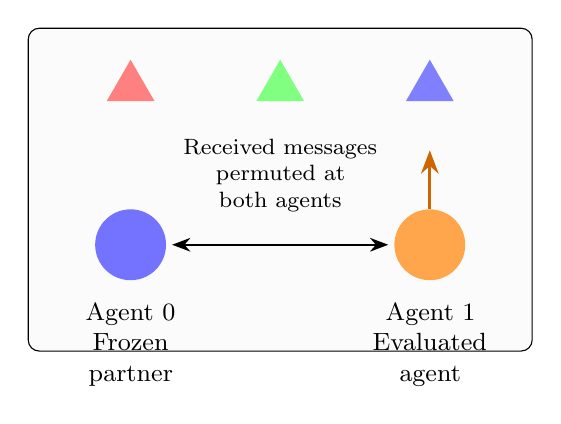
\begin{tikzpicture}[>=Stealth,font=\small]
\draw[rounded corners,fill=gray!3] (0,0) rectangle (6.4,4.1);
\node[circle,fill=blue!55,minimum size=9mm,inner sep=0pt] (a) at (1.3,1.35) {};
\node[circle,fill=orange!70,minimum size=9mm,inner sep=0pt] (b) at (5.1,1.35) {};
\node[align=center,text width=2cm,anchor=north] at (1.3,.73) {Agent 0\\Frozen partner};
\node[align=center,text width=2cm,anchor=north] at (5.1,.73) {Agent 1\\Evaluated agent};
\foreach \x/\col in {1.3/red,3.2/green,5.1/blue}{\node[regular polygon,regular polygon sides=3,fill=\col!50,minimum size=7mm,inner sep=0pt] at (\x,3.35) {};}
\draw[<->,thick,shorten <=2pt,shorten >=2pt] (a.east) -- (b.west);
\node[align=center,text width=2.6cm,anchor=south,font=\footnotesize] at (3.2,1.65) {Received messages\\permuted at both agents};
\draw[->,very thick,orange!80!black] (b.north) -- (5.1,2.55);
\end{tikzpicture}
\end{minipage}\hfill
\begin{minipage}[c]{0.38\linewidth}
\raggedright\small
\textbf{Semantic intervention}\\[3pt]
Relabel received symbols at both agents.
\par\vspace{12pt}
\textbf{Motor intervention}\\[3pt]
Rotate movement commands of agent 1 only.
\end{minipage}
\caption{Task schematic, not a measured trajectory. The intervention scope is asymmetric: messages change at both receivers, while only the controlled agent's actuator rotates. Landmarks and positions are illustrative.}
\label{fig:task}
\end{figure}

\subsection{Four conditions}
Each evaluation session lasts 60 episodes, with a change point $\tau$ sampled beforehand between 12 and 35, inclusive. The task is nominal before $\tau$. From episode $\tau$ onward, we apply no change, a received-message permutation, a fixed clockwise rotation of agent 1's movement commands, or both. The rotation preserves no-op. The ten-symbol permutation changes at least one symbol but may leave others unchanged; it remains fixed within the session and affects both receivers. The policy is not given the condition, permutation, or change point.

The movement intervention changes command effects, not the teammate's strategy. Separating the two interfaces also does not equalize difficulty: identifying a ten-symbol relabelling may require different evidence and more interaction than identifying a fixed rotation.

\section{Selective adaptation (V2)}
V2 has three components: a pretrained policy that chooses movements and messages, a separate neural module that interprets received messages, and a motor module that estimates how commands affect motion. The two correction modules do \emph{not} share neural weights. In fact, the motor module estimates an action mapping rather than using a second neural network. During evaluation, neural weights stay fixed; adaptation changes recurrent memories, detection statistics and the motor mapping.

\subsection{Base policy and message correction}
The base policy is a recurrent MAPPO actor trained on the nominal task, then frozen. It has separate output heads for movement and outgoing messages. The receiver module is a separate 128-unit gated recurrent unit (GRU), trained to estimate what an incoming message would have been in the original communication code. It outputs a distribution over the ten original symbols and a confidence that the code has changed.

For example, suppose an intervention relabels incoming symbol 2 as symbol 7. The receiver module tries to recover the original symbol 2 from the observed symbol 7 and the interaction history. It is not told the permutation during evaluation. Its estimate can be uncertain, so it supplies a probability distribution rather than necessarily choosing a single symbol.

The receiver module has 38 inputs: the local observation (21), previous own movement (5) and message (10), previous reward divided by five (1), and an episode-reset indicator (1). Each previous action uses a one-hot vector: one entry is 1 at the chosen action's index and all others are 0. Original symbols and change labels supervise this module during training only. Its recurrent memory persists across episodes within a session, allowing evidence about the code to accumulate. The base policy's recurrent states reset at every episode.

A binary gate $g_e$ decides whether episode $e$ uses message correction. For the raw received vector $m_t$ and the estimated original-code distribution $\hat m_t$,
\begin{equation}
 \tilde m_t=(1-g_e)m_t+g_e\hat m_t.
\end{equation}
Thus $g_e=0$ passes the received message unchanged, while $g_e=1$ replaces it with the estimate. Only the message entries of the observation are replaced. The all-zero vector at the start of an episode denotes no incoming message and remains zero.

\subsection{Two uses of the same base policy}
The frozen actor is evaluated twice at each step, with separate recurrent states. One pass receives the corrected observation and supplies the movement decision. The other receives the raw observation and supplies the outgoing message. These two passes share the base actor's weights; they are not the semantic and motor correction modules described above.

This design prevents receiver correction from directly changing the outgoing-message computation for the same raw observation history. Movement changes can still affect later observations and therefore later messages. The restriction also has a cost: repairing how agent 1 interprets incoming symbols does not repair how agent 0 interprets agent 1's outgoing symbols. In our message-change condition, both receivers are perturbed, but only agent 1 can adapt.

\subsection{Motor correction from observed motion}
The motor module compares commanded movements with their observed effects. It fits a least-squares velocity predictor using the first 100 transitions. For each subsequent transition, it compares the observed next velocity with predictions for all five commands. Three consecutive prediction errors above $0.05$ activate correction. Decayed command--effect counts and a linear assignment then give an inverse action mapping.

For example, if the environment turns an intended upward command into rightward motion, correction selects the command estimated to produce upward motion instead. The module applies this remapping to the base policy's movement probabilities; it does not modify messages or neural weights. It is never given the true rotation. Direct velocity feedback and a small set of candidate effects make this fixed-rotation task particularly suitable for the module.

\subsection{When message correction is enabled or withdrawn}
The semantic gate requires both sustained loss of return and confidence in a code change. The first eight episodes establish a baseline using their median return and median absolute deviation (MAD), with the scale floored at 3. A cumulative statistic accumulates evidence of lower returns. Activation requires this statistic to cross a threshold, three consecutive degraded episodes, and mean episode confidence of at least $0.8$. The threshold is calibrated on training-side no-change data and stays fixed during evaluation.

After activation, a four-episode trial checks whether returns have worsened beyond a variance-dependent margin. If so, the gate disables message correction and waits eight episodes before allowing reactivation. We call this withdrawal \emph{rollback}; it switches off correction rather than restoring or retraining neural weights. These safeguards seek to avoid unnecessary intervention, but they can delay useful correction. Motor correction has its own transition-based detector and does not wait for the semantic gate.

\begin{figure}[ht]
\centering
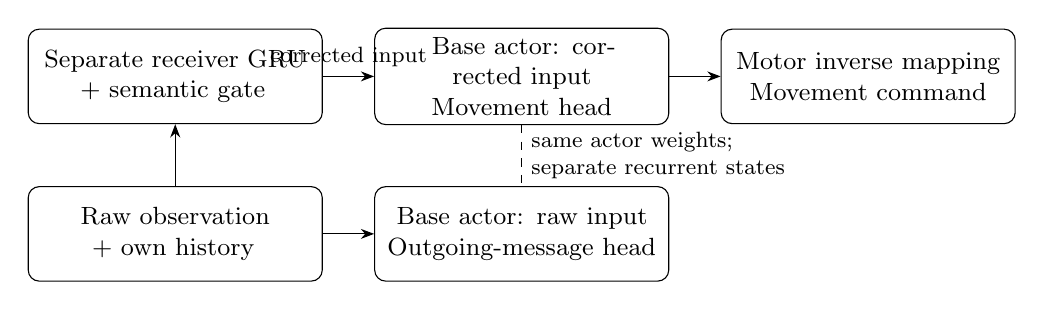
\begin{tikzpicture}[>=Stealth,box/.style={draw,rounded corners,align=center,font=\small,text width=3.5cm,minimum height=12mm}]
\node[box] (memory) at (0,0) {Separate receiver GRU\\+ semantic gate};
\node[box] (move) at (4.4,0) {Base actor: corrected input\\Movement head};
\node[box] (motor) at (8.8,0) {Motor inverse mapping\\Movement command};
\node[box] (raw) at (0,-2) {Raw observation\\+ own history};
\node[box] (sender) at (4.4,-2) {Base actor: raw input\\Outgoing-message head};
\draw[->] (raw)--(memory);
\draw[->] (memory)-- node[above,font=\footnotesize]{corrected input} (move);
\draw[->] (move)--(motor);
\draw[->] (raw)--(sender);
\draw[dashed] (move)-- node[right,align=left,font=\footnotesize]{same actor weights;\\separate recurrent states} (sender);
\end{tikzpicture}
\caption{V2 execution. Message correction acts before the policy's movement decision; motor correction remaps that decision afterward. The sender uses the raw observation. The receiver GRU has its own weights, separate from the base actor. Neural weights are fixed at evaluation; memories, detectors and the motor mapping evolve.}
\end{figure}

\section{Experimental design}
\subsection{Separate comparison campaigns}
The completed selectivity-control campaign contains five training seeds, eleven methods, four conditions, and twenty sessions per combination. It includes frozen, motor-only, joint, unguarded, confidence-only, reward-only, no-rollback, shared-stream, continued-MAPPO and randomized-MAPPO controls. Its two-agent adaptation interface differs from the LIAM comparison. These scores are not pooled.

A training seed defines an independently trained set of models. Each set is tested in multiple sessions; a session contains 60 episodes and one fixed intervention schedule. The LIAM campaign originally planned five training seeds and seven methods. On 29 September 2026, it was closed with seeds 1--3 because of access problems and the project deadline, after these results had already been inspected. Seed 4 was interrupted and seed 5 was not completed. This is a disclosed deviation from the original protocol, not a prespecified three-seed study. All methods control only agent 1; agent 0 uses the same frozen recurrent MAPPO partner for a given training seed. Partner actions have their own seeded random generator. World/session seeds are paired across methods. The V2 actor and memory are held fixed across conditions within a seed. Weights differ across training seeds. Each method/condition has twenty sessions of sixty episodes. Training sessions use a separate seed range, 48 episodes, balanced condition cycling and a change point between 10 and 30.

\paragraph{What the seven methods test.}
Frozen uses the base policy without correction. Motor only adds the motor mapping. Selective V2 uses both modules with the gate described above. Joint V2 also enables message correction when the motor detector activates, testing whether both corrections should be triggered together. Unguarded V2 enables message correction after the eight-episode warm-up without rollback. These V2 variants retain the motor detector. LIAM 3.42M and LIAM 40M are the earlier and later checkpoints of the same LIAM training run. The simpler V2 variants test whether selective activation adds value beyond the corrections themselves.

\subsection{LIAM port and resources}
The official source is pinned to revision \texttt{8545b9e4237eb60ad45b7cb8ed6caec6bc4263b5}. Imported A2C, reconstruction, storage and normalization methods are unchanged. The bridge resizes observations to 21 and the two action components to five and ten. The policy loss does not update the context encoder; its representation is learned through the reconstruction objective. The released configuration supplies hidden size 128, embedding size 20, actor/representation learning rates $3\cdot10^{-4}$/$7\cdot10^{-4}$, entropy coefficient $.01$, value coefficient $.5$, discount $.99$ and GAE $.95$. Training uses five consecutive five-step chunks per episode.

There are substantial protocol differences from the original LIAM experiment: MPE2 observations/dynamics, a ten-symbol channel, one pretrained partner per seed, and 32 rather than ten vector environments. At a fixed interaction count, this last choice changes the number of optimizer updates. This is a task port, not a numerical replication of the paper. LIAM's recurrent state resets each episode, while V2's semantic memory persists across episodes.

The prespecified LIAM checkpoints are 3,420,800 and 40,000,000 learner steps. The first equals V2's recorded 2,998,400 base-training plus 422,400 memory/validation/calibration interactions. It is only a learner-budget comparison: LIAM also needs the pretrained partner, whereas the V2 actors were jointly trained. Supervision differs as well: LIAM receives partner reconstruction targets during training, and V2 receives clean-symbol/change targets. These asymmetries prevent an architecture-only efficiency conclusion.

\subsection{Measures and planned inference}
For a session with change point $\tau$, pre-change return averages the five preceding episodes and post-change return averages all remaining episodes. The no-change condition uses the same artificial split. We average sessions within each training seed, then report the mean and sample standard deviation across training seeds. Episodes and sessions are not treated as independent training replications.

The prespecified primary criterion compares V2 with LIAM at 40M steps: positive paired differences in all three changed conditions with one-sided paired $t$ tests and Holm correction, plus no-change noninferiority using a one-sided 95\% lower bound above $-0.25$. The original criterion required all five seeds. It is not evaluated in this closed three-seed report, and no confirmatory success or failure is assigned. Three seeds provide very limited precision. Earlier-checkpoint and other comparisons are descriptive. Pre-change competence and unnecessary no-change interventions must also be reported.

\section{Results of the closed three-seed study}
\subsection{Published-method comparison: three completed seeds}
Table~\ref{tab:partial} reports only seeds 1--3. Each cell first averages twenty sessions per seed. Table~\ref{tab:seeds} exposes the training variability hidden by aggregate means. No confirmatory result is claimed from this partial subset.
\begin{table}[ht]
\centering\small
\caption{Post-change team return, mean $\pm$ training-seed SD ($n=3$). Higher is better. One controlled agent with a common frozen partner.}
\label{tab:partial}
\begin{tabular}{lrrrr}\toprule
Method & No change & Messages & Movement & Both \\\midrule
Frozen & $-8.11 \pm 0.14$ & $-19.49 \pm 0.81$ & $-22.57 \pm 0.66$ & $-28.17 \pm 0.79$ \\
Motor only & $-8.11 \pm 0.14$ & $-19.49 \pm 0.81$ & $-9.01 \pm 0.03$ & $-20.17 \pm 0.89$ \\
Joint V2 & $-8.11 \pm 0.14$ & $-18.50 \pm 0.70$ & $-9.08 \pm 0.06$ & $-18.98 \pm 0.73$ \\
Unguarded V2 & $-8.15 \pm 0.11$ & $-18.11 \pm 0.77$ & $-9.07 \pm 0.06$ & $-18.87 \pm 0.83$ \\
Selective V2 & $-8.11 \pm 0.14$ & $-18.50 \pm 0.70$ & $-9.01 \pm 0.03$ & $-19.13 \pm 0.79$ \\
LIAM 3.42M & $-29.89 \pm 6.14$ & $-30.21 \pm 5.67$ & $-28.56 \pm 3.85$ & $-28.92 \pm 3.02$ \\
LIAM 40M & $-15.52 \pm 6.42$ & $-19.40 \pm 2.96$ & $-16.08 \pm 5.96$ & $-19.46 \pm 2.92$ \\
\bottomrule\end{tabular}
\end{table}

\begin{table}[ht]
\centering\small
\caption{Individual training seeds. Pre-change return is identical across conditions within a method/seed because the pre-change trajectories are paired.}
\label{tab:seeds}
\begin{tabular}{clrrrrr}\toprule
Seed & Method & Pre-change & No change & Messages & Movement & Both \\\midrule
1 & V2 & -7.56 & -8.00 & -18.85 & -9.03 & -19.55 \\
1 & LIAM 40M & -10.63 & -11.29 & -17.92 & -12.22 & -18.08 \\
2 & V2 & -7.78 & -8.26 & -17.70 & -9.00 & -18.22 \\
2 & LIAM 40M & -11.97 & -12.37 & -17.47 & -13.09 & -17.48 \\
3 & V2 & -7.53 & -8.06 & -18.97 & -8.98 & -19.62 \\
3 & LIAM 40M & -23.41 & -22.90 & -22.81 & -22.94 & -22.81 \\
\bottomrule\end{tabular}
\end{table}

V2 has a higher aggregate post-change mean in every condition, but LIAM obtains higher message-only and combined-change returns in seeds 1 and 2. LIAM seed 3 is already weak before the change. Consequently, the aggregate semantic comparison is sensitive to initial competence and training instability; it is not evidence that V2 recovers faster. V2 makes no applied corrections in the 60 no-change sessions across these three seeds and reproduces its frozen-policy performance there. This supports preservation of nominal behaviour on these sessions, not absence of false alarms in general.

The V2--LIAM gap is approximately $7.42$ return units without a change and $7.08$ under motor rotation. Thus the higher motor-condition return cannot be attributed entirely to a greater adaptation benefit: much of the advantage is already present in nominal competence. Conversely, the gap shrinks to about $0.89$ under message permutation. To measure adaptation benefit, we must also compare how much each method loses or recovers after the same change, and how much recovery is possible when the true correction is supplied.

Within this same one-controlled-agent comparison, unguarded V2 exceeds selective V2 by approximately $0.392$ on messages and $0.268$ on combined changes, while selective V2 exceeds it by $0.048$ without change and $0.066$ on movement. These descriptive differences are consistent with a protection--recovery trade-off, but they do not isolate the detector's mechanism. Motor-only correction essentially matches selective V2 on the movement condition, so motor success should not be attributed to the semantic gate.

\begin{figure}[ht]
\centering
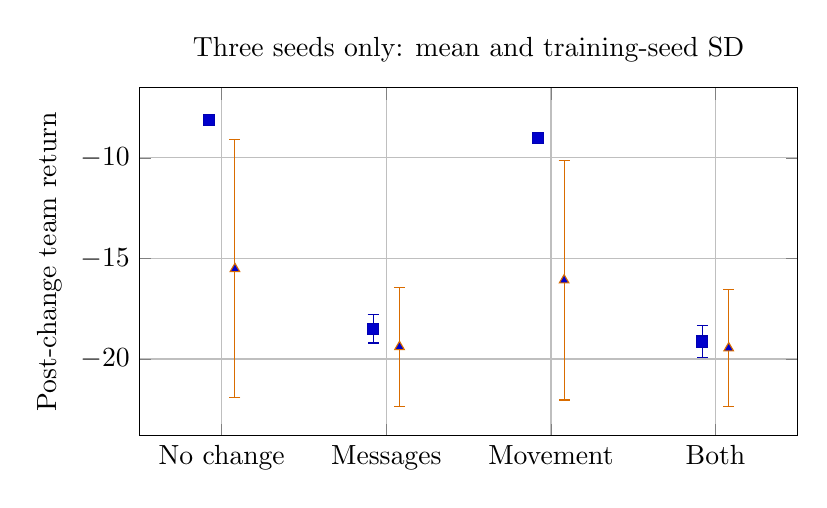
\begin{tikzpicture}\begin{axis}[width=.82\textwidth,height=6cm,xmin=-.5,xmax=3.5,xtick={0,1,2,3},xticklabels={No change,Messages,Movement,Both},ylabel={Post-change team return},grid=major,title={Three seeds only: mean and training-seed SD}]
\addplot+[only marks,forget plot,color=blue!70!black,mark=square*,error bars/.cd,y dir=both,y explicit] coordinates {(-0.08,-8.1055) +- (0,0.1390)};
\addplot+[only marks,forget plot,color=blue!70!black,mark=square*,error bars/.cd,y dir=both,y explicit] coordinates {(0.92,-18.5046) +- (0,0.7027)};
\addplot+[only marks,forget plot,color=blue!70!black,mark=square*,error bars/.cd,y dir=both,y explicit] coordinates {(1.92,-9.0070) +- (0,0.0265)};
\addplot+[only marks,forget plot,color=blue!70!black,mark=square*,error bars/.cd,y dir=both,y explicit] coordinates {(2.92,-19.1341) +- (0,0.7885)};
\addplot+[only marks,forget plot,color=orange!85!black,mark=triangle*,error bars/.cd,y dir=both,y explicit] coordinates {(0.08,-15.5207) +- (0,6.4153)};
\addplot+[only marks,forget plot,color=orange!85!black,mark=triangle*,error bars/.cd,y dir=both,y explicit] coordinates {(1.08,-19.3969) +- (0,2.9640)};
\addplot+[only marks,forget plot,color=orange!85!black,mark=triangle*,error bars/.cd,y dir=both,y explicit] coordinates {(2.08,-16.0827) +- (0,5.9564)};
\addplot+[only marks,forget plot,color=orange!85!black,mark=triangle*,error bars/.cd,y dir=both,y explicit] coordinates {(3.08,-19.4591) +- (0,2.9188)};
\end{axis}\end{tikzpicture}
\caption{Blue squares: V2; orange triangles: LIAM 40M port. Error bars are sample SD across three training seeds, not confidence intervals. Individual values are in Table~\ref{tab:seeds}.}
\end{figure}

\begin{figure}[ht]
\centering
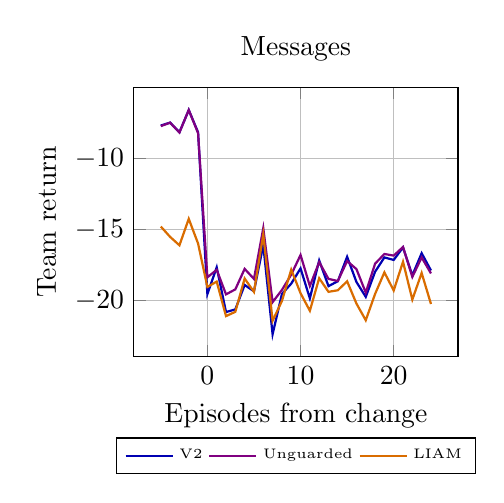
\begin{tikzpicture}\begin{axis}[width=.47\textwidth,height=5cm,xlabel={Episodes from change},ylabel={Team return},title={Messages},grid=major,legend style={font=\tiny,at={(.5,-.3)},anchor=north,legend columns=3}]
\addplot[thick,color=blue!70!black] coordinates {(-5,-7.6928) (-4,-7.4869) (-3,-8.1685) (-2,-6.5999) (-1,-8.1654) (0,-19.5442) (1,-17.6628) (2,-20.8084) (3,-20.6195) (4,-18.9056) (5,-19.3455) (6,-16.1070) (7,-22.3724) (8,-19.5390) (9,-18.8080) (10,-17.7397) (11,-19.8450) (12,-17.1781) (13,-18.9878) (14,-18.6385) (15,-16.9217) (16,-18.6924) (17,-19.7405) (18,-17.9746) (19,-16.9671) (20,-17.1436) (21,-16.2594) (22,-18.2256) (23,-16.6697) (24,-17.8839)};\addlegendentry{V2}
\addplot[thick,color=violet] coordinates {(-5,-7.7334) (-4,-7.4921) (-3,-8.1795) (-2,-6.6002) (-1,-8.2234) (0,-18.3681) (1,-17.8371) (2,-19.5637) (3,-19.2130) (4,-17.7720) (5,-18.4781) (6,-14.9071) (7,-20.1116) (8,-19.2546) (9,-18.1753) (10,-16.7930) (11,-18.9780) (12,-17.2986) (13,-18.4748) (14,-18.6259) (15,-17.2208) (16,-17.7876) (17,-19.4418) (18,-17.4095) (19,-16.7248) (20,-16.8394) (21,-16.2327) (22,-18.3356) (23,-16.9673) (24,-18.0929)};\addlegendentry{Unguarded}
\addplot[thick,color=orange!85!black] coordinates {(-5,-14.7959) (-4,-15.5214) (-3,-16.1137) (-2,-14.2534) (-1,-15.9876) (0,-19.0460) (1,-18.6657) (2,-21.0932) (3,-20.7901) (4,-18.4505) (5,-19.3922) (6,-15.3553) (7,-21.4212) (8,-20.0342) (9,-17.8254) (10,-19.4822) (11,-20.7171) (12,-18.4283) (13,-19.3864) (14,-19.2750) (15,-18.6480) (16,-20.2098) (17,-21.3851) (18,-19.5367) (19,-18.0183) (20,-19.2923) (21,-17.2694) (22,-19.9301) (23,-18.0605) (24,-20.2413)};\addlegendentry{LIAM}
\end{axis}\end{tikzpicture}
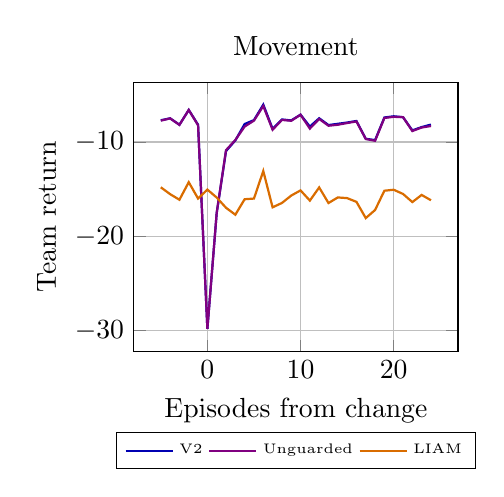
\begin{tikzpicture}\begin{axis}[width=.47\textwidth,height=5cm,xlabel={Episodes from change},ylabel={Team return},title={Movement},grid=major,legend style={font=\tiny,at={(.5,-.3)},anchor=north,legend columns=3}]
\addplot[thick,color=blue!70!black] coordinates {(-5,-7.6928) (-4,-7.4869) (-3,-8.1685) (-2,-6.5999) (-1,-8.1654) (0,-29.8044) (1,-17.5296) (2,-10.9584) (3,-9.8298) (4,-8.0910) (5,-7.6753) (6,-6.0344) (7,-8.5960) (8,-7.6060) (9,-7.7108) (10,-7.0959) (11,-8.3614) (12,-7.4822) (13,-8.2002) (14,-8.0682) (15,-7.9334) (16,-7.7710) (17,-9.6532) (18,-9.7969) (19,-7.3985) (20,-7.2716) (21,-7.3647) (22,-8.7657) (23,-8.4165) (24,-8.1515)};\addlegendentry{V2}
\addplot[thick,color=violet] coordinates {(-5,-7.7334) (-4,-7.4921) (-3,-8.1795) (-2,-6.6002) (-1,-8.2234) (0,-29.8029) (1,-17.4937) (2,-10.8604) (3,-9.7833) (4,-8.3597) (5,-7.7295) (6,-6.1827) (7,-8.6965) (8,-7.6589) (9,-7.7445) (10,-7.1096) (11,-8.5744) (12,-7.5540) (13,-8.2718) (14,-8.1689) (15,-7.9858) (16,-7.8167) (17,-9.6775) (18,-9.8658) (19,-7.4477) (20,-7.3276) (21,-7.3629) (22,-8.8337) (23,-8.4608) (24,-8.3024)};\addlegendentry{Unguarded}
\addplot[thick,color=orange!85!black] coordinates {(-5,-14.7959) (-4,-15.5214) (-3,-16.1137) (-2,-14.2534) (-1,-15.9876) (0,-15.0412) (1,-15.8784) (2,-16.9651) (3,-17.7018) (4,-16.0611) (5,-15.9895) (6,-13.0713) (7,-16.9175) (8,-16.4576) (9,-15.6717) (10,-15.1235) (11,-16.2052) (12,-14.8121) (13,-16.4624) (14,-15.8704) (15,-15.9419) (16,-16.3370) (17,-18.0592) (18,-17.2034) (19,-15.1565) (20,-15.0571) (21,-15.5011) (22,-16.3611) (23,-15.6048) (24,-16.1712)};\addlegendentry{LIAM}
\end{axis}\end{tikzpicture}
\caption{Raw episode-return curves aligned to the first changed episode. Each point averages twenty sessions within each seed, then the three seeds equally. All sessions contain this $[-5,24]$ window. No smoothing or uncertainty inference is applied. The curves include differences in initial policy competence.}
\end{figure}

\subsection{Exploratory uncertainty}
For transparency, Table~\ref{tab:uncertainty} reports unadjusted paired Student-$t$ intervals over the three training-seed differences, with two degrees of freedom. These intervals are descriptive, have very limited precision, and do not replace the unfulfilled five-seed confirmatory protocol. All four intervals include zero. Neither the mean ranking nor these intervals establish equivalence or general superiority.
\begin{table}[ht]
\centering
\caption{V2 minus LIAM 40M post-change return, three paired training seeds. Intervals are exploratory and not multiplicity-adjusted.}
\label{tab:uncertainty}
\begin{tabular}{lrr}\toprule
Condition & Mean difference & Exploratory 95\% interval \\\midrule
No change & 7.415 & $[-8.601,23.431]$ \\
Messages & 0.892 & $[-5.512,7.296]$ \\
Movement & 7.076 & $[-7.778,21.929]$ \\
Both & 0.325 & $[-5.897,6.547]$ \\\bottomrule
\end{tabular}
\end{table}


\subsection{Completed simpler-control campaign}
In the separate five-seed, two-adaptive-agent campaign, V2 obtained message-only return $-18.152\pm0.615$, compared with $-17.638\pm0.805$ for unguarded correction; movement-only return was $-9.041\pm0.099$, compared with $-8.994\pm0.065$ for motor-only correction. The prespecified selectivity-superiority criterion failed. These results are retained as negative evidence against a blanket claim that selective routing improves return. They are not entries in the LIAM table and cannot be used as matched comparisons to LIAM.

\section{Why movement and communication differ}
\paragraph{Verified structural differences.}
Motor identification receives immediate local evidence: a selected command and the next velocity. The intervention is a fixed one-to-one remapping of a few movement commands, exactly the type of change this adapter is designed to invert. Message correction must instead infer what a symbol refers to from incomplete observations and the interaction history. The semantic gate can wait several episodes, whereas motor evidence accumulates at individual transitions. A movement mismatch can therefore be detected from a single step, while evidence about an incorrect message interpretation may take several episodes.

The intervention affects both message receivers, but only one agent can adapt in the LIAM campaign. Correcting the controlled agent's incoming message does not directly repair its partner's incoming channel. V2 additionally preserves its raw sender stream. LIAM conditions both action heads on a learned context, which could permit compensatory outgoing communication. This is a plausible mechanism, not a measured account of LIAM's learned strategy. The return is a team average, so residual partner failure matters.

\paragraph{Evidence versus explanation.}
The simpler-control results are consistent with conservative gating trading semantic recovery for protection against unnecessary intervention. They do not isolate gating delay, decoder accuracy, or partner compensation. The archived LIAM-comparison metrics count any applied correction per episode; they do not record separate gate onset, confidence, rollback, decoding accuracy or agent-specific return. The aligned curves therefore cannot by themselves establish which mechanism caused the observed ordering. A model need not explicitly separate semantics and movement to represent both in its latent state.

\paragraph{Prospective diagnostic experiments.}
An oracle control is given the true intervention, providing an upper bound on what a correction could repair. A new diagnostic campaign should use fresh seeds and a protocol fixed in advance, containing: (1) unilateral versus bilateral message permutation, holding the evaluated agent and partner fixed; (2) oracle message inversion at the controlled receiver, then at both receivers, to estimate repair ceilings; (3) oracle gate with the same learned decoder, separating routing error from decoding error; (4) learned gate with oracle decoder, separating the reverse contribution; and (5) sender-preserving versus sender-adaptive policies under equal training resources. Log onset delays, motor prediction error, canonical decoding quality, message frequencies, per-agent returns and false interventions. These experiments are proposed, not completed, and must not modify or tune against the closed evaluation dataset.

\section{Limitations and reproducibility}
The evidence covers one small cooperative environment, one fixed actuator rotation and message permutations; it does not establish general robustness to nonstationary teammates. Intervention severity and scope are unequal. The policy families, interaction budgets, training privileges, recurrent horizons and optimization schedules differ. The original LIAM benchmark has not been reproduced. Three seeds are insufficient for the planned five-seed conclusion, and a low-performing seed must not be discarded because it changes the ranking.

Appendix~\ref{app:audit} records artifact checks, implementation tests and the interrupted runs. Appendix~\ref{app:psc} develops the proposed Relay Workshop task and the PSC extensions needed to support it; neither is part of the experiments reported here.

\section{Conclusion}
This preliminary study separates evidence for a useful motor correction from evidence for selective routing and semantic adaptation. The current system provides a concrete, inspectable decomposition and strong movement recovery in the tested setting, but has not established superiority of selective adaptation. The central research opportunity is to determine when mechanism-specific correction is identifiable and when preserving a communication component prevents joint recovery. The original five-seed comparison remains unfulfilled. Prospective diagnostic controls and additional independent evidence would be needed for stronger claims.

\appendix
\section{Reproducibility and interrupted runs}\label{app:audit}
The recovered local archive preserves the frozen protocol, source snapshot, dependencies, training logs, checkpoint hashes, session metrics and episode returns. All three training status files record completion at 40 million steps and all three evaluation completion markers are present. The six LIAM checkpoint hashes match the server manifest, as does the source snapshot; eight partner/memory manifest entries were also verified, for 15 matching hash entries in total. Across 1,680 sessions and 100,800 episodes, we verified complete record keys, finite returns, paired scenario seeds/change points, and pre/post summaries recalculated from raw episodes. The recovered evaluation files exactly match those used in the earlier figures. This audit validates the recovered artifacts; it does not reproduce the original LIAM paper's benchmark scores.

Additional implementation tests verify exact action/value initialization and optimizer-update equivalence with the imported core at matching configurable dimensions, gradient isolation, and equality of training/evaluation trajectories and team rewards. Recovered model checkpoints permit inference but lack the complete optimizer, normalizer and random-generator state needed for exact training continuation.

An interruption occurred in seed 4 at 24,800,800 steps. Its checkpoint lacked optimizer, return-normalization and random-generator states. The interrupted run was preserved and the same seed restarted from scratch with the unchanged 40M-step protocol; seed 5 was scheduled afterward but was not completed. The partial run is not used to select a favourable checkpoint. The restarted seed 4 was later interrupted at a last recorded 7,440,800 steps. The institutional systems team subsequently confirmed termination of processes for excessive compute use during teaching hours. This confirms administrative process interruption, but does not establish the cause of every observed filesystem-permission change. On 29 September 2026 the study was closed because no time remained for further training. The report retains only the three complete evaluations, including the weak third LIAM seed, and discloses the unfulfilled five-seed plan. Future intensive jobs on these servers must respect the institution's night/weekend restrictions.


\section{Future environments and the PSC engine}\label{app:psc}

The scientific question is not whether an environment can be constructed in which our adapter wins. It is whether the benefits of separating communication correction and action correction depend predictably on observability, intervention scope, and coupling between the two mechanisms. The current negative routing result motivates this question rather than invalidating it. A useful benchmark must admit both favourable and unfavourable regimes for modular adaptation.

Our implemented contribution combines an existing recurrent MAPPO policy, a supervised recurrent receiver estimator, online motor system identification, and conservative activation/rollback. MAPPO supplies the base optimizer \cite{yu2022}; LIAM supplies an independently published local-information comparator \cite{papoudakis2021}. MPE2 supplies the existing particle task \cite{mpe2}. Our contributions are the intervention harness, adapter composition, controlled comparisons and diagnosis. Neither the policy optimizer nor the particle simulator is claimed as original. Explicit module separation is not evidence of disentangled learned representations.

\subsection{Proposed game: Relay Workshop}

Relay Workshop is a proposed cooperative grid game, not an implemented environment or an established novelty claim. Two robots must deliver a specified component to the correct workbench and perform the requested operation. An inspector sees the work order, but not the carrier's local obstacles; a carrier sees nearby passages, tools and objects, but not the private order. They communicate using a finite symbol channel. At the next episode their roles can be exchanged. This design makes both communication and control useful without making success require our specific adapter architecture.

A first version uses a 7-by-7 grid, three component types, three benches, at most two obstacles, and at most 50 joint decision steps. Actions include four moves, wait, pick up, and deliver; a separate communication component selects a symbol or silence. An episode ends at successful delivery or timeout. The primary reward is one for correct completion, zero otherwise, with a small fixed step cost documented separately. Shaping, if used during training, must be identical across baselines and excluded from the primary success metric. These are proposed starting settings, to be checked for solvability rather than adopted as a finished protocol.

Four intervention families are crossed: no change, communication only, control only, and both. Communication changes relabel a specified directed channel, initially one receiver only. Control changes remap the same receiver's movement commands. The comparison then expands to both receivers and both actuators, so the scope asymmetry in our current MPE2 experiment becomes an explicit factor. Mild symbol swaps and axis swaps precede larger permutations; recurrent switches and noisy actions form later stress tests. Game layouts, task identities and switch schedules have held-out splits. The canonical alphabet and actuator mapping are hidden from all evaluated learners.

Crucially, movement effects are locally observable, whereas order meanings need evidence from interaction. A calibration zone can vary the amount of grounding evidence available equally to all methods. To test the limits of modularity, a coupled variant makes a communicated operation depend on the tool currently held. In that variant, a context-independent symbol translator may be inadequate. A strong shared-context baseline should be allowed to win.

\subsection{Falsifiable hypotheses and controls}

\par\noindent H1: independent, locally identifiable shifts favour targeted correction in sample efficiency or recovery delay, at matched nominal competence and resources.
\par\noindent H2: receiver-only correction becomes insufficient when the unadapted partner's channel also changes; sender adaptation or joint correction reduces that deficit.
\par\noindent H3: conservative routing reduces unnecessary interventions but increases recovery delay when semantic evidence is weak.
\par\noindent H4: increasing semantic-action coupling reduces the advantage of independent modules, possibly reversing it.

Compare a frozen policy, always-on adapters, selective adapters, a learned shared-context model with matched capacity, a matched recurrent policy trained on randomized contexts, and the ported LIAM baseline. Include oracle channel inversion and oracle actuator inversion as repair ceilings, clearly separated from deployable methods. Match available history, training information and interaction budgets where feasible; report remaining mismatches. A shared representation baseline is needed because LIAM differs from V2 in more than separation alone.

First validate nominal solvability with scripted planners and centralized-information upper bounds. Require each learned baseline to reach a prespecified nominal competence range before interpreting adaptation rankings. This threshold must be fixed on validation tasks, with a rule for reporting methods that fail it, not used to discard inconvenient final seeds. Compare success rate, episode return, recovery delay, unnecessary interventions, affected/unaffected module changes, and held-out generalization. Record both per-agent outcomes and team outcomes. Define a held-out primary contrast after pilot feasibility checks and before the final test. Retain difficult or failed conditions rather than redesigning the test to ensure V2 wins.

\subsection{Existing environments as complementary tests}

Overcooked offers an established cooperative coordination setting \cite{carroll2019}. It is useful for testing joint planning and role coordination, but explicit relabelled communication would be an extension, not a claim about the original benchmark. Hanabi offers partial information and constrained communication \cite{bard2019}; it could test semantic conventions, but is less directly suited to physical actuator shifts. An additional established benchmark helps distinguish a method's generality from advantages engineered into Relay Workshop. Neither environment has been ported or evaluated in this project.

\subsection{PSC: present capabilities and required extensions}

The current PSC repository contains a C\#/WPF grid editor, scripted rules, persistent game documents, local playtesting and transition-tree analysis. Its core contracts are separated from the user interface, but the editor currently targets two-player placement/alignment games. It does not yet provide the MARL training backend, partial-observation interface, simultaneous robot actions, or Python environment bridge required by Relay Workshop. The MPE2 experiments reported above were not run inside PSC.

The proposed extension has five deliverables: a headless deterministic runner; agent-specific observation and action contracts; a seeded intervention scheduler separate from game rules; a Python adapter following an appropriate PettingZoo interface \cite{terry2021}; and replay/telemetry exports showing exactly what changed. For joint decisions, collect both actions before one world transition; if an alternating-turn interface is chosen instead, expose its timing explicitly. The WPF editor can author layouts and inspect replays while the headless core runs on Linux for training. That portability requires implementation and tests; it is not an existing feature claim.

Version each experiment as a game specification, observation specification, intervention specification and seed manifest. Keep privileged labels in an evaluator-only log, separate from learner observations. Verify deterministic replay, absence of observation leakage, action validity, episode termination and identical results between interactive and headless runs. A recorded intervention should permit comparison with a no-change run from the same initial state and random seed.

The defensible PSC positioning is therefore: \textbf{a proposed engine for authoring and inspecting controlled multi-agent adaptation experiments}. A later software contribution could demonstrate that users can build several environments, reproduce runs, and isolate failure mechanisms. The present manuscript can introduce this direction, but claims about usability, throughput or generality require completed implementations and measurements. Keep benchmark-engineering evidence distinct from algorithm-superiority evidence.

The cited environments motivate future extensions; they are not additional tested baselines. The originality of Relay Workshop and the broader engine contribution remains to be established through a dedicated related-work review.

\begin{thebibliography}{9}
\bibitem{lowe2017} R. Lowe, Y. Wu, A. Tamar, J. Harb, P. Abbeel, and I. Mordatch. Multi-Agent Actor-Critic for Mixed Cooperative-Competitive Environments. NeurIPS, 2017. \url{https://arxiv.org/abs/1706.02275}.
\bibitem{yu2022} C. Yu, A. Velu, E. Vinitsky, J. Gao, Y. Wang, A. Bayen, and Y. Wu. The Surprising Effectiveness of PPO in Cooperative Multi-Agent Games. NeurIPS, 2022. \url{https://arxiv.org/abs/2103.01955}.
\bibitem{papoudakis2021} G. Papoudakis, F. Christianos, and S. V. Albrecht. Agent Modelling under Partial Observability for Deep Reinforcement Learning. NeurIPS, 2021. \url{https://arxiv.org/abs/2006.09447}.
\bibitem{liamcode} Papoudakis et al. Official LIAM implementation. Revision \texttt{8545b9e4237eb60ad45b7cb8ed6caec6bc4263b5}, MIT license. \url{https://github.com/uoe-agents/LIAM}.
\bibitem{mpe2} Farama Foundation. MPE2, Simple Reference environment documentation. Accessed 29 September 2026. \url{https://mpe2.farama.org/environments/simple_reference/}.
\bibitem{carroll2019} M. Carroll et al. On the Utility of Learning about Humans for Human-AI Coordination. NeurIPS, 2019. \url{https://arxiv.org/abs/1910.05789}.
\bibitem{bard2019} N. Bard et al. The Hanabi Challenge: A New Frontier for AI Research. Preprint, 2019. \url{https://arxiv.org/abs/1902.00506}.
\bibitem{terry2021} J. K. Terry et al. PettingZoo: A Standard API for Multi-Agent Reinforcement Learning. NeurIPS, 2021. \url{https://arxiv.org/abs/2009.14471}.
\end{thebibliography}
\end{document}
